\chapter{XML}

\section{Arbre}

Voici un exemple d'arbre XML illustrant les données manipulées pour ce projet.

\xml
\begin{lstlisting}
<?xml version = "1.0" encoding="UTF-8" standalone="yes" ?>
<annuaire>
	<annuaire_id>Id</annuaire_id>
	<categorie categorie_id ="Id" name="categorie">
		<annonce>
			<annonce_id>Id</annonce_id>
			<nom>Nom</nom>
			<adresse>
				<adresse_id>Id</adresse_id>
				<rue>Rue</rue>
				<ville>Ville</ville>
				<codepostal>00000</codepostal>
			</adresse>
			<telephone>0000000000</telephone>
		</annonce>
		<annonce>
			<annonce_id>Id</annonce_id>
			<nom>Nom</nom>
			<adresse>
				<adresse_id>Id</adresse_id>
				<rue>Rue</rue>
				<ville>Ville</ville>
				<codepostal>00000</codepostal>
			</adresse>
			<telephone>0000000000</telephone>
		</annonce>
	</categorie>
	<categorie categorie_id ="Id" name="categorie">
		<annonce>
			<annonce_id>Id</annonce_id>
			<nom>Nom</nom>
			<adresse>
				<adresse_id>Id</adresse_id>
				<rue>Rue</rue>
				<ville>Ville</ville>
				<codepostal>00000</codepostal>
			</adresse>
			<telephone>0000000000</telephone>
		</annonce>
	</categorie>
</annuaire>
\end{lstlisting}
Et voici sa représentation graphique sous forme d'arbre :
\begin{figure}[H]
    \centering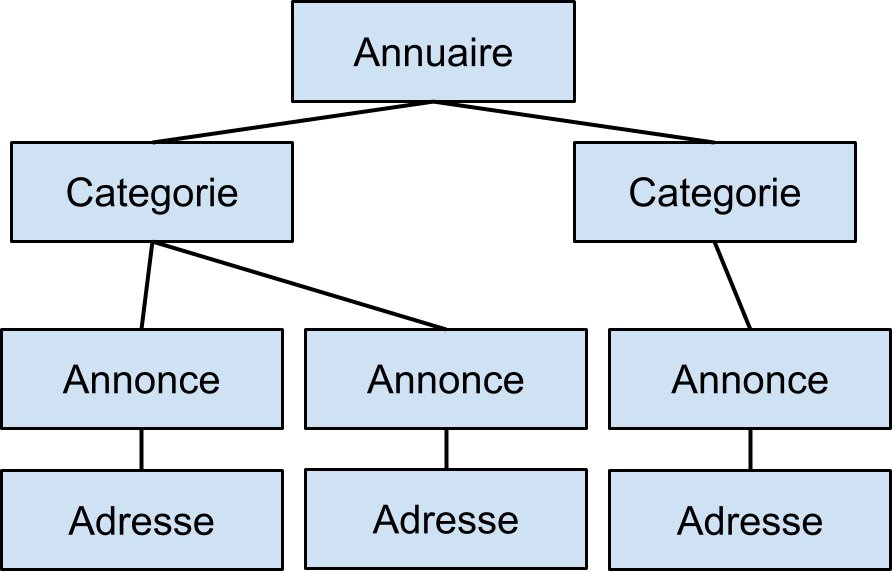
\includegraphics[width=.7\textwidth]{images/arbre.png}
    \caption{Arbre de l'XML}
\end{figure}

\section{Schéma XML}

Voici le schéma XSD correspond à notre XML :

\begin{lstlisting}
<?xml version="1.0" encoding="UTF-8" ?>
<xs:schema attributeFormDefault="unqualified" elementFormDefault="qualified" xmlns:xs="http://www.w3.org/2001/XMLSchema">
  <xs:element name="annuaire">
    <xs:complexType>
      <xs:sequence>
        <xs:element type="xs:string" name="annuaire_id"/>
        <xs:element name="categorie" maxOccurs="unbounded" minOccurs="0">
          <xs:complexType>
            <xs:sequence>
              <xs:element name="annonce" maxOccurs="unbounded" minOccurs="0">
                <xs:complexType>
                  <xs:sequence>
                    <xs:element type="xs:string" name="annonce_id"/>
                    <xs:element type="xs:string" name="nom"/>
                    <xs:element name="adresse">
                      <xs:complexType>
                        <xs:sequence>
                          <xs:element type="xs:string" name="adresse_id"/>
                          <xs:element type="xs:string" name="rue"/>
                          <xs:element type="xs:string" name="ville"/>
                          <xs:element type="xs:byte" name="codepostal"/>
                        </xs:sequence>
                      </xs:complexType>
                    </xs:element>
                    <xs:element type="xs:byte" name="telephone"/>
                  </xs:sequence>
                </xs:complexType>
              </xs:element>
            </xs:sequence>
            <xs:attribute type="xs:string" name="categorie_id" use="optional"/>
            <xs:attribute type="xs:string" name="name" use="optional"/>
          </xs:complexType>
        </xs:element>
      </xs:sequence>
    </xs:complexType>
  </xs:element>
</xs:schema>
\end{lstlisting}

\chapter{Conception}
\section{Diagramme de classes}

\begin{figure}[H]
    \centering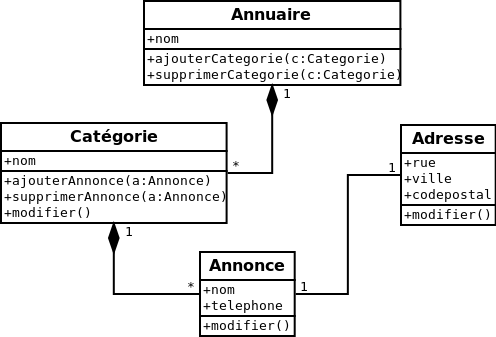
\includegraphics[width=.8\textwidth]{images/UML.png}
    \caption{Diagramme de classes (UML)}
\end{figure}

\section{Diagramme logique de données (MLD)}

\fakeshell
\begin{lstlisting}
Annuaire(#nom:string)
Categorie(#nom:string, #annuaire=>Annuaire(nom))
Annonce(#nom:string, #categorie=>Categorie(nom), adresse=>Adresse(adresse_id), telephone:string)
Adresse(#adresse_id:integer, rue:string, ville:string, codepostal:string)
\end{lstlisting}

\chapter{Web service}

\section{Interface : prototypes des méthodes}

Nous avons décidé de créer deux webservices :

\begin{itemize}
    \item Un pour l'application cliente d'administration (création, modification et suppression des catégories et annonces)
    \item Un pour l'application cliente de recherche d'annonces
\end{itemize}

Voici le webservice d'administration :

\java
\begin{lstlisting}
String createCategory(String name)

String deleteCategorie(int categorie_id)

String updateCategorie(int categorie_id, String name)

String getAllCategorie()

String getCategory(int category_id)

String createAd(String name, int categorie_id, String rue, String ville, String codepostal, String telephone)

String deleteAd(int annonce_id)

String updateAd(int annonce_id, String name, int categorie_id, String rue, String ville, String codepostal, String telephone)

String getAllAd()

String getAd(int annonce_id)
\end{lstlisting}
Et voici le webservice pour la recherche d'annonces :
\begin{lstlisting}
String getByParams(String name, String categoryName, String street, String city, String postcode)
\end{lstlisting}
Pour nos deux webservices, chaque fonction retourne une \lstinline{String} au format JSON.

\section{Messages SOAP}

\subsection{Requête}

Voici une requête faite depuis l'application cliente de recherche d'annonces, vers le serveur :

\xml
\begin{lstlisting}
<?xml version="1.0" encoding="UTF-8"?>
<soapenv:Envelope xmlns:soapenv="http://schemas.xmlsoap.org/soap/envelope/" xmlns:xsd="http://www.w3.org/2001/XMLSchema" xmlns:xsi="http://www.w3.org/2001/XMLSchema-instance">
	<soapenv:Body>
		<getByParams xmlns="http://webservice">
			<name>ad</name>
			<categoryName xsi:nil="true"/>
			<street xsi:nil="true"/>
			<city>paris</city>
			<postcode xsi:nil="true"/>
		</getByParams>
	</soapenv:Body>
</soapenv:Envelope>
\end{lstlisting}

\subsection{Réponse}

Et voici la réponse à cette requête. Nous retournons du JSON qui est encapsulé dans du XML automatiquement.

\begin{lstlisting}
<?xml version="1.0" encoding="utf-8"?>
<soapenv:Envelope xmlns:soapenv="http://schemas.xmlsoap.org/soap/envelope/" xmlns:xsd="http://www.w3.org/2001/XMLSchema" xmlns:xsi="http://www.w3.org/2001/XMLSchema-instance">
	<soapenv:Body>
		<getByParamsResponse xmlns="http://webservice">
			<getByParamsReturn>
                [{&quot;annonce_id&quot;:1,&quot;nom&quot;:&quot;ad11&quot;,&quot;categorie_id&quot;:8,&quot;adresse_id&quot;:1,&quot;telephone&quot;:&quot;0251&quot;,&quot;categorieObjet&quot;:{&quot;categorie_id&quot;:8,&quot;nom&quot;:&quot;cat2358&quot;},&quot;adresseObjet&quot;:{&quot;adresse_id&quot;:1,&quot;rue&quot;:&quot;rue&quot;,&quot;ville&quot;:&quot;paris&quot;,&quot;codepostal&quot;:&quot;85&quot;}},{&quot;annonce_id&quot;:2,&quot;nom&quot;:&quot;ad2&quot;,&quot;categorie_id&quot;:1,&quot;adresse_id&quot;:2,&quot;telephone&quot;:&quot;0251&quot;,&quot;categorieObjet&quot;:{&quot;categorie_id&quot;:1,&quot;nom&quot;:&quot;cat1&quot;},&quot;adresseObjet&quot;:{&quot;adresse_id&quot;:2,&quot;rue&quot;:&quot;rue&quot;,&quot;ville&quot;:&quot;parisss&quot;,&quot;codepostal&quot;:&quot;85&quot;}}]
			</getByParamsReturn>
		</getByParamsResponse>
	</soapenv:Body>
</soapenv:Envelope>
\end{lstlisting}

\chapter{Architecture}

\begin{figure}[H]
    \centering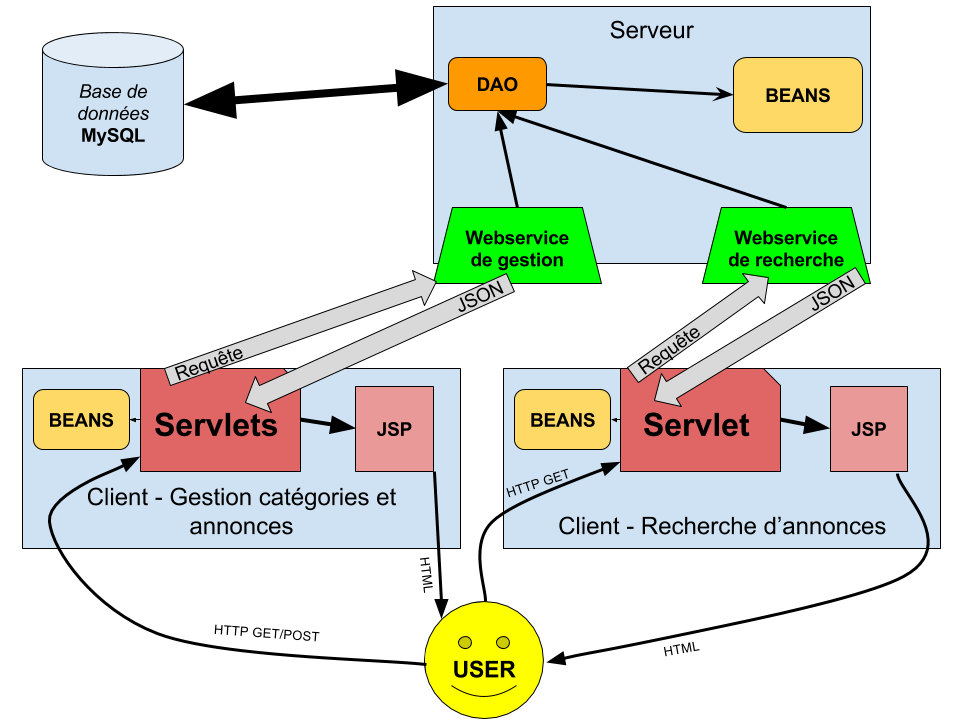
\includegraphics[width=1\textwidth]{images/archi.png}
    \caption{Architecture de l'application}
\end{figure}

Un utilisateur peut utiliser deux applications web (qui tournent sur Tomcat) au choix:
\begin{itemize}
  \item Une application web de gestion de l'annuaire, où il peut créer, modifier et supprimer des catégories. Il peut également faire la même chose avec des annonces.
  \item Une application web de consultation où il peut voir l'ensemble des annonces ou alors faire des recherches sur les annonces pour en trouver seulement certaines, répondant à des critères de recherche.
\end{itemize}

Lorsqu'il accède à l'une des deux applications, voici ce qu'il se passe :

\begin{enumerate}
  \item Il envoit une requête HTTP à l'application web pour accèder à une page.
  \item Selon les paramètres contenus dans la requête (qui peut être de type GET ou POST), la servlet va soit simplement renvoyer une page HTML générée à partir d'une page JSP, soit faire des traitements plus poussés en utilisant l'API (webservice) de notre serveur, puis renvoyer du HTML généré à partir d'une JSP et de la réponse de l'API.
  \item Dans le cas où la servlet a besoin d'utilisateur le web service, elle va utiliser un objet de la classe \lstinline{Proxy} (en appelant une méthode sur cet objet). De manière transparente, une requête est faite sur le serveur, qui tourne aussi sur Tomcat.
  \item La fonction du webservice qui est appelée va instancier une ou plusieurs DAO.
  \item Les DAO utilisent les \lstinline{Beans}, qui sont une représentation des tables SQL que nous avons créées. Les DAO vont donc faire des requêtes SQL et instancier des objets \lstinline{Beans} à partir des résultats de la requête SQL.
  \item La fonction du webservice initialement appelée récupère les résultats produits par la ou les DAO et les sérialise en JSON.
  \item Le JSON est retourné à la servlet.
  \item La servlet désérialise le JSON et instancie des \lstinline{Beans}. Ces derniers, souvent sous forme de listes, sont transmis à la JSP qui va produire le HTML renvoyé au client.
\end{enumerate}
